\subsection{General Concepts}\label{ch:general-concepts}
%What is a Conf. system and why we use it
We call a software system configurable if it offers options that allow developers to select functionality to change the behavior of the system. %Maybe more to which degree
By this, the system can satisfy the demand of multiple user groups. 
While we provide only a single software system that include various features for users to choose from~\cite{TooManyKnobs}.


\begin{figure}[h]
    \centering
    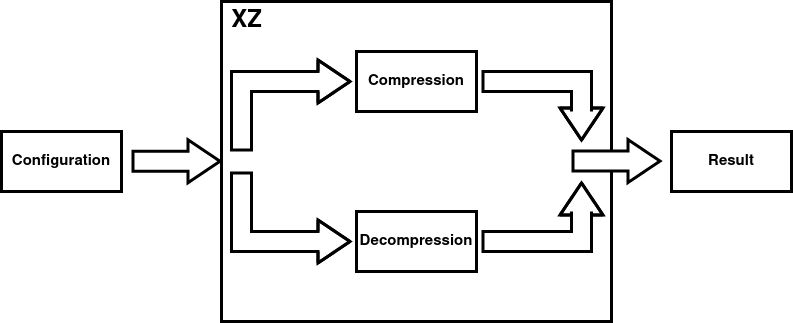
\includegraphics[scale=0.55]{gfx/ConfigurableSystemXZ.png}
    \caption{Simplified version of \textsc{XZ}.}
    \label{fig:xz}
\end{figure}

%Example for such a system using xz
As an example, let us inspect the compression tool \textsc{XZ}\footnote{Visited at 21.03.2023 \url{https://tukaani.org/xz/}}.
\autoref{fig:xz} depicts a simplified version of \textsc{XZ}, which contains two main functions: compression and decompression. 
It is up to the user to decide what he needs, for when he wants to compress a file he would select a configuration that enables this functionality,
but regardless the choice, the software system contains both functions.
